
\documentclass[11pt,a4paper]{article}
\usepackage{indentfirst}   %% 首行缩进
\usepackage{fontspec, xunicode, xltxtra, verbatim}
\usepackage{listings}      %% 支持代码
\usepackage{xcolor}        %% 代码颜色
\usepackage{supertabular}  %% 打表格
%\setmainfont{Microsoft YaHei}
%\setmainfont{FangSong}  
\setmainfont{SimSun}       %% 字体

\XeTeXlinebreaklocale zh   %% 中文自动换行
\XeTeXlinebreakskip = 0pt plus 1pt
\parindent 2em             %% 段落缩进
\linespread{1.2}           %% 行间距


\author{王大伟}
\title{情感词及其极性识别}
\begin{document} 

%% 包含代码的全局设置
\lstset{numbers=left, 
numberstyle= \tiny, 
keywordstyle= \color{ blue!70},commentstyle=\color{red!50!green!50!blue!50}, 
frame=shadowbox, 
rulesepcolor= \color{ red!20!green!20!blue!20} 
} 

\maketitle
\begin{center}
班级:Z1303322
学号:1130332040
\end{center}

\newpage

\tableofcontents
\newpage

\section{问题}

自动识别出100个文本集中所包含的情感词和极性,即在一定的上下文环境中能够明确表达观点的倾向性词语,以及该情感词的极性(正面(褒义)或者负面(贬义))。

输出结果要求按照置信度排序(可自己设计置信度计算模型),且仅输出置信度最高的前100个情感词和它们的极性(注意:若一个情感词在不同的文本或者同一文本中出现了多次,只需输一个个结果即可)。

同时,要求给出情感词所在文本的编号,以及以情感词为中心、前后各20个字节组成的文本片段,用于之处情感词出现的位置以消除评测时可能产生的歧义。

\section{需求分析}

词语级的情感极性分析是句子级和篇章级的情感极性分析的基础和前提,它包括2个方面的含义:提取出可能具有情感倾向的候选词;对该候选词进行分析,判断其倾向性及极性强度。中文文本的情感词一般以形容词、动词、名词、副词为主。词语的情感极性计算主要有2 种方法:基于词典的方法和基于语料库的方法。

本文描述的主要是基于词典的方法,主要是利用词典中词语之间的相互联系来挖掘情感词。英文中常用的方法是计算情感词与种子词在Wordnet中的关联程度来识别出情感词;中文中常用的词典是知网(HowNet),取得了较好的效果。


\subsection{算法描述}

\begin{enumerate}
\item 准备好语料文档,使用NLPIR/ICTCLAS2014分词系统对语料进行中文分词,并标注词性,如:/v 表示动词, /a 表示形容词等。
\item 中文文本的情感词一般以形容词、动词、名词、副词为主,从分词序列中抽取这些类型的词语,并使用Hownet的正面情感词词典计算该词的正向相似度(psim);使用Hownet的负面情感词词典计算该词的负向相似度(nsim)。词语的语义相似度算法,可参见文献[4](本文附件里面的代码实现了该算法的C++版封装)。
\item 抽取该词的上下文环境里面的关联词(表示递进、并列、转折关系)或否定词。如:"不"、"不是"等。
\item 根据词语的正向相似度和负向相似度,及其上下文中的关联词和否定词,来确定该词的情感极性。
\item 跳转到第二步,直到所有的词语极性都得以计算。
\item 根据置信度排序,输出结果。
\end{enumerate}

\subsection{系统框架图}

\begin{figure}[!hbp]
\centering
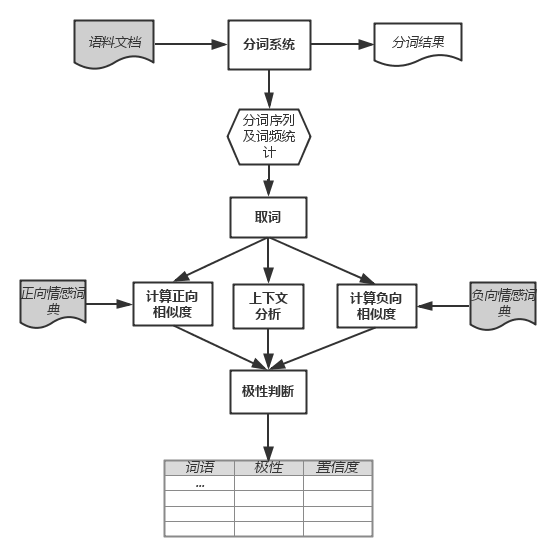
\includegraphics[width=0.9\textwidth]{sentiment.png}
\caption{系统框架图}
\end{figure}

\clearpage

\section{设计与实现}

下面将逐一介绍上述系统框架图中的各个部分的设计和部分实现代码。

\subsection{分词系统}

NLPIR分词系统前身为2000年发布的ICTCLAS词法分析系统,从2009年开始,为了和以前工作进行大的区隔,并推广NLPIR自然语言处理与信息检索共享平台,调整命名为NLPIR分词系统。张华平博士先后倾力打造十余年,内核升级十余次,先后获得了2010年钱伟长中文信息处理科学技术奖一等奖,2003年国际SIGHAN分词大赛综合第一名,2002年国内973评测综合第一名。全球用户突破30万,包括中国移动、华为、中搜、3721、NEC、中华商务网、硅谷动力、云南日报等企业,清华大学、新疆大学、华南理工、麻省大学等机构:同时,ICTCLAS广泛地被《科学时报》、《人民日报》海外版、《科技日报》等多家媒体报道。

附件中的程序把语料文档通过ICTCLAS分词系统,转化成带词性标注的结果文件,同时把词语以下面的结构保存在内存中,并统计了词频,方便PMI和SOPMI的计算(本文未采用该方式)。\vspace{6pt}

{\scriptsize\begin{lstlisting}[language=C] 
struct DocWord
{
  std::string word;  // 词
  int start;         // 文档中的开始位置
  int length;        // 长度
  int type;          // 词性类型(nlpir_wordtype.h)
};
\end{lstlisting}}

分词的程序如下:\vspace{6pt}

{\scriptsize\begin{lstlisting}[language=C] 
bool SentimentParser::loadMaterials()
{
  // 初始化分词组件
  if(!NLPIR_Init(NLPIR_DATA_DIR, UTF8_CODE))
  {
    util::log("[ERROR] ICTCLAS init failed.");
    return false;
  }

  NLPIR_SetPOSmap(ICT_POS_MAP_SECOND);
 
  // 对文件进行分词
  for (size_t i = 1; i <= 100; i++)
  {
    char srcfile[128] = "";
    char dstfile[128] = "";
    snprintf(srcfile, sizeof(srcfile), "%s/%ld.txt", MATERIAL_SRC_PATH, i);
    snprintf(dstfile, sizeof(dstfile), "%s/%ld.txt", MATERIAL_DST_PATH, i);

    // 生成分词结果文件
    NLPIR_FileProcess(srcfile, dstfile, 1);

    // 生成分词内存结构
    std::string content;
    loadFile(srcfile, content);
    wordParse(i, content);
  }

  // 释放分词组件资源
  NLPIR_Exit();
  return true;
}
\end{lstlisting}}

\subsection{基于Hownet计算词的语义相似度}

在《知网》中,是通过用一系列的义原,利用某种知识描述语言来描述一个概念。而这些义原通过上下位关系组织成一个树状义原层次体系。我们的目标是要找到一种方法,对用这种知识描述语言表示的两个语义表达式进行相似度计算。

下面大概介绍一下语义相似的计算方法,详情参见文献[4]。

\subsubsection{词语相似度计算}

对于两个汉语词语$W_{1}$和$W_{2}$,如果$W_{1}$有$n$个义项(概念):$S_{11}$,$S_{12}$,\ldots{},$S_{1n}$,$W_{2}$有$m$个义项(概念):$S_{21}$,$S_{22}$,\ldots{},$S_{2m}$,我们规定,$W_{1}$和$W_{2}$的相似度是各个概念的相似度之最大值,也就是说:

\[
Sim(W_{1},W_{2})=\max_{i=1..n,j=1..m}Sim(S_{1i},S_{2j})
\]

这样,我们就把两个词语之间的相似度问题归结到了两个概念之间的相似度问题。当然,我们这里考虑的是孤立的两个词语的相似度。如果是在一定上下文之中的两个词语,最好是先进行词义排歧,将词语标注为概念,然后再对概念计算相似度。

\subsubsection{义原相似度计算}

由于所有的概念都最终归结于用义原(个别地方用具体词)来表示,所以义原的相似度计算是概念相似度计算的基础。

由于所有的义原根据上下位关系构成了一个树状的义原层次体系,我们这里采用简单的通过语义距离计算相似度的办法。假设两个义原在这个层次体系中的路径距离为$d$,根据上面的公式,我们可以得到这两个义原之间的语义距离:

\[
Sim(p_{1}, p_{2})=\frac{\alpha}{d + \alpha}
\]

其中$p_{1}$和$p_{2}$表示两个义原(primitive),$d$是$p_{1}$和$p_{2}$在义原层次体系中的路径长度,是一个正整数。$\alpha$是一个可调节的参数。

\subsubsection{虚词概念的相似度的计算}

我们认为,在实际的文本中,虚词和实词总是不能互相替换的,因此,虚词概念和实词概念的相似度总是为零。

\subsubsection{实词概念的相似度的计算}

《知网》的知识描述语言可以通过义原和集合、特征结构这两种抽象数据结构来表达。义原之间的相似度计算问题已经解决,剩下的问题就是集合和特征结构的相似度问题了。

我们的基本设想是:整体相似要建立在部分相似的基础上。把一个复杂的整体分解成部分,通过计算部分之间的相似度得到整体的相似度。

假设两个整体A和B都可以分解成以下部分:$A$分解成$A_{1}$,$A_{2}$,\ldots{},$A_{n}$,$B$分解成$B_{1}$,$B_{2}$,\ldots{},$B_{m}$,那么这些部分之间的对应关系就有$m x n$种。问题是:这些部分之间的相似度是否都对整体的相似度发生影响?如果不是全部都发生影响,那么我们应该如何选择发生影响的那些部分之间的相似度?选择出来以后,我们又如何得到整体的相似度?

我们认为:一个整体的各个不同部分在整体中的作用是不同的,只有在整体中起相同作用的部分互相比较才有效。例如比较两个人长相是否相似,我们总是比较它们的脸型、轮廓、眼睛、鼻子等相同部分是否相似,而不会拿眼睛去和鼻子做比较。

因此,在比较两个整体的相似性时,我们首先要做的工作是对这两个整体的各个部分之间建立起一一对应的关系,然后在这些对应的部分之间进行比较。


在《知网》中对一个实词的描述可以表示为一个特征结构,该特征结构含有以下四个特征:
\begin{itemize}
\item 第一基本义原描述: 其值为一个基本义原,我们将两个概念的这一部分的相似度记为$Sim_{1}(S_{1},S_{2})$;

\item 其它基本义原描述:对应于语义表达式中除第一基本义原描述式以外的所有基本义原描述式,其值为一个基本义原的集合,我们将两个概念的这一部分的相似度记为$Sim_{2}(S_{1},S_{2})$;

\item 关系义原描述: 对应于语义表达式中所有的关系义原描述式,其值是一个特征结构,对于该特征结构的每一个特征,其属性是一个关系义原,其值是一个基本义原,或一个具体词。我们将两个概念的这一部分的相似度记为$Sim_{3}(S_{1},S_{2})$;

\item 关系符号描述:对应于语义表达式中所有的关系符号描述式,其值也是一个特征结构,对于该特征结构的每一个特征,其属性是一个关系义原,其值是一个集合,该集合的元素是一个基本义原,或一个具体词。我们将两个概念的这一部分的相似度记为$Sim_{4}(S_{1},S_{2})$。
\end{itemize}

于是,两个概念语义表达式的整体相似度记为:

\[
Sim(S_{1}, S_{2}) = \sum_{i=1}^4 \beta_{i}Sim_{i}(S_{1}, S_{2})
\]

其中,$\beta_{i}(1\leq i \leq 4)$是可调节的参数,且有:

\[
\beta_{1} + \beta_{2} + \beta_{3} + \beta_{4} = 1, \beta_{1} \geq \beta_{2} \geq \beta_{3} \geq \beta_{4}
\]

后者反映了$Sim_{1}$到$Sim_{4}$对于总体相似度所起到的作用依次递减。由于第一基本义原描述式反映了一个概念最主要的特征,所以我们应该将其权值定义得比较大,一般应在$0.5$以上。

在实验中我们发现,如果$Sim_{1}$非常小,但$Sim_{3}$或者$Sim_{4}$比较大,将导致整体的相似度仍然比较大的不合理现象。因此我们对上面的公式进行了修改,得到公式如下:

\[
Sim(S_{1}, S_{2}) = \sum_{i=1}^4 \beta_{i}\prod_{j=1}^i Sim_{j}(S_{1}, S_{2})
\]

其意义在于,主要部分的相似度值对于次要部分的相似度值起到制约作用,也就是说,如果主要部分相似度比较低,那么次要部分的相似度对于整体相似度所起到的作用也要降低。且可以保证一个词和它本身的相似度仍为1。

\subsubsection{计算词语相似度的程序}

具体实现参加similarity.h/cpp,用法如下:\vspace{6pt}

{\scriptsize\begin{lstlisting}[language=C] 
WordSimilarity::instance()->init();
WordSimilarity::instance()->calc("十分", "犀利");
\end{lstlisting}}

\subsection{极性判断}

\subsubsection{正向相似度和负向相似度}


正向相似度的计算:

\[
Sim_{p} = \max_{i=1..m}\{Sim(W, P_{i})\}
\]

其中$W$是要计算的词,$P_{i}$是Hownet正向情感词表中的第$i$个词。


正向相似度的计算:

\[
Sim_{n} = \max_{i=1..n}\{Sim(W, N_{i})\}
\]

其中$W$是要计算的词,$N_{i}$是Hownet负向情感词表中的第$i$个词。

代码如下:\vspace{6pt}

{\scriptsize\begin{lstlisting}[language=C]

float SentimentParser::calcSimilarityWordAndSet(const std::string& word, 
  const WordSet& wordset)
{
  if (0 == word.length() || wordset.empty())
    return 0.0;

  float sim = 0.0;
  for (WordSet::iterator it = wordset.begin();  it != wordset.end(); ++ it)
  {
    float similarity = WordSimilarity::instance()->calc(word, (*it));
    if (similarity > 0.0)
    {
      if (similarity > sim)
        sim = similarity;
    }
  }

  return sim;
}

float psim = calcSimilarityWordAndSet(i->first, pset_); // 正向相似度
float nsim = calcSimilarityWordAndSet(i->first, nset_); // 负向相似度
\end{lstlisting}}


\subsubsection{计算词的情感极性}

由$Sim_{p}$和$Sim_{n}$来计算词的情感极性。规则如下:

\begin{center}
\begin{tabular}{|c|c|l|}
\hline
条件 & 情感极性 & 备注 \\
\hline
$Sim_{p}\leq\alpha$, $Sim_{n}\leq\alpha$ & 中性 & $\alpha$为相似度阈值,本文中设置为0.5\\
\hline
$|Sim_{p}-Sim_{n}|<\beta$ & 中性 & 与Pset和Nset相似距离差不多 \\
\hline
$Sim_{p}/Sim_{n} > 1$ & 正向 & 与Pset更相似 \\
\hline
$Sim_{n}/Sim_{p} > 1$ & 负向 & 与Nset更相似 \\
\hline
\end{tabular}
\end{center}

其对应代码如下:\vspace{6pt}

{\scriptsize\begin{lstlisting}[language=C]

int SentimentParser::calsWordSentiment(float psim, float nsim)
{
  if (psim < COEFF_ALPHA && nsim < COEFF_ALPHA)
    return 0;

  if (psim == nsim)
    return 0;

  if (psim / nsim > COEFF_BELTA)
    return 1;
  else if (nsim / psim > COEFF_GAMMA)
    return -1;

  return 0;
}

int type = calsWordSentiment(psim, nsim);               // 极性

\end{lstlisting}}

\subsubsection{由上下文环境决定极性强度}

根据词所在的上下文中的关联词和否定词来进一步确定词的情感极性。

\begin{itemize}
\item 否定词主要有:“不”、“不是”等。
\item 关联词分为三种类型:
\begin{enumerate}
\item[1)] 递进关联词,例如,“而且”、“更加”、“甚至”等;
\item[2)] 并列关联词,例如,“也”、“并”、“又”等;
\item[3)] 转折关联词,例如,“但是”、“不过”、“只是”等。
\end{enumerate}
\end{itemize}

\section{调试分析}


开发环境:

基于linux/cygwin环境,用C++开发,使用了NLPIR/ICTCLAS2014分词系统,和自己根据文献[4]实现了一个基于hownet的词汇相似度计算工具。\vspace{6pt}

附件程序介绍:

\begin{enumerate}
\item 源码结构 

\begin{itemize}
\item utility.h         - 一些功能函数 
\item similarity.h/cpp  - 相似度计算工具
\item sentiment.h/cpp   - 情感词识别
\item main.cpp          - 主函数入口
\item Makefile          - 可以在linux/cygwin环境下使用 
\end{itemize}

\item 应用相关

\begin{itemize}
\item app               - 生成的可执行文件目录
\item app\_data          - 语料100篇所在目录
\item app\_data\_result   - 语料100篇分词后的结果,和top100.txt(根据置信度排序的100个情感词)
\end{itemize}

\item 知网相关

\begin{itemize}
\item hownet            - hownet义原表和词典所在目录
\item pset.txt          - hownet正向情感词典
\item nset.txt          - hownet负向情感词典
\end{itemize}

\item NLPIR/ICTCLAS2014相关

\begin{itemize}
\item include           - NLPIR.h头文件目录
\item lib               - 库文件目录
\item Data              - NLPIR的数据目录
\end{itemize}

\end{enumerate}

编译:

\begin{itemize}
\item make     - 编译可执行文件
\item make sim - 编译相似度计算器
\end{itemize}

执行:

\begin{itemize}
\item  run.bat  - windows
\item  run.sh   - linux/cygwin
\end{itemize}

执行结果:

\begin{itemize}
\item  app\_data\_result/top100.txt - 根据置信度排序的100个情感词
\item  app\_data\_result/1.txt..    - 语料分词后的结果
\end{itemize}

\section{测试结果}

\subsection{词语相似度计算结果}

由下表可以看到,绝大部分结果还是比较合理的,但也有部分结果不够合理,例如“中国”和“联合国”、“中国”和“安理会”的相似度都过低,这是因为,“中国”、“联合国”、“安理会”在《知网》中的第一基本义原分别是“地方”、“机构”、“部件”。“跑”和“跳”的相似度也较低,这是因为这两个词被简单定义为两个基本义原,而缺少其它信息。这也从一个侧面反映了知网的某些定义不合理或不一致之处。

\begin{center}
{\scriptsize\begin{tabular}{|l|l|l|c|l|l|l|}
\hline
词语1 & 词语2 & 相似度 && 词语1 & 词语2 & 相似度 \\
\hline
男人 & 女人 & 0.800000 && 男人 & 父亲 & 1.000000 \\
\hline
男人 & 母亲 & 0.800000 && 男人 & 和尚 & 0.800000 \\
\hline
男人 & 经理 & 0.579200 && 男人 & 高兴 & 0.044444 \\
\hline
男人 & 收音机 & 0.107758 && 男人 & 鲤鱼 & 0.208696 \\
\hline
男人 & 苹果 & 0.171429 && 男人 & 工作 & 0.126316 \\
\hline
男人 & 责任 & 0.126316 && 工人 & 教师 & 0.589600 \\
\hline
工人 & 科学家 & 0.575926 && 工人 & 农民 & 0.600000 \\
\hline
工人 & 运动员 & 0.579200 && 教师 & 科学家 & 0.577563 \\
\hline
教师 & 农民 & 0.589600 && 教师 & 运动员 & 0.579200 \\
\hline
科学家 & 农民 & 0.575926 && 科学家 & 运动员 & 0.579200 \\
\hline
农民 & 运动员 & 0.579200 && 中国 & 美国 & 0.833333 \\
\hline
中国 & 联合国 & 0.127405 && 中国 & 安理会 & 0.092133 \\
\hline
中国 & 欧洲 & 0.764000 && 粉红 & 红 & 1.000000 \\
\hline
粉红 & 红色 & 1.000000 && 粉红 & 绿 & 0.800000 \\
\hline
粉红 & 颜色 & 0.054637 && 绿 & 颜色 & 0.054637 \\
\hline
十分 & 非常 & 1.000000 && 十分 & 特别 & 0.600000 \\
\hline 
思考 & 考虑 & 1.000000 && 思考 & 思想 & 0.074074 \\
\hline
跑 & 跳 & 0.444444 && 跑 & 跳舞 & 0.126984 \\
\hline
\end{tabular}}
\end{center}


\subsection{情感词极性结果}

由下表可见大部分词语的情感极性都是正确的,正向情感词的置信度直接取了$psim$,负向情感词的置信度直接取了$nsim$。有部分词语情感极性并不是特别明显,如“逛”,“安装”等,主要是因为这些词的hownet义原与情感词种子词典有部分重叠;还有下面的结果没有考虑词的上下文,所以整个方案还需要进一步改进,才能提高情感词的识别率和准确性。

\begin{center}
\scriptsize{\begin{supertabular}{|l|l|l|l|l|l|l|}
\hline
序号 & 学号 & 词 & 文档 & 极性 & 上下文 & 置信度 \\
\hline
1 & 1130332040 & 安装 & Doc43 & pos &  1.5at锋范,安装了导航和后视 & 1.000000 \\
\hline
2 & 1130332040 & 寻找 & Doc25 & neg & 。可是我真的想寻找一下知音 & 1.000000 \\
\hline
3 & 1130332040 & 希望 & Doc14 & pos & 害是不小的。只希望这些东东 & 1.000000 \\
\hline
4 & 1130332040 & 帮助 & Doc14 & pos & 虎tt的朋友有所帮助。转载:c & 1.000000 \\
\hline
5 & 1130332040 & 帮忙 & Doc46 & pos &  求大神帮忙!12款307行车电脑 & 1.000000 \\
\hline
6 & 1130332040 & 延迟 & Doc1 & pos & 的反应,感觉有延迟。看论坛 & 1.000000 \\
\hline
7 & 1130332040 & 开启 & Doc29 & pos & 不给力的。由于开启空调需要 & 1.000000 \\
\hline
8 & 1130332040 & 徘徊 & Doc5 & neg & 19万。 这样我就徘徊在两个车 & 1.000000 \\
\hline
9 & 1130332040 & 忽悠 & Doc7 & neg & 换了,结果被js忽悠了老p7  真 & 1.000000 \\
\hline
10 & 1130332040 & 怠 & Doc14 & neg & 扭力,在发动机怠速下它是不 & 1.000000 \\
\hline
11 & 1130332040 & 感激 & Doc26 & pos & 不算贵了~不慎感激~ & 1.000000 \\
\hline
12 & 1130332040 & 感谢 & Doc60 & pos & 。  最后要特别感谢一下瑞丰4 & 1.000000 \\
\hline
13 & 1130332040 & 指望 & Doc21 & pos & ”做的事,不要指望了,所谓 & 1.000000 \\
\hline
14 & 1130332040 & 挑选 & Doc21 & pos & 菱悦的时候可以挑选3年或10万 & 1.000000 \\
\hline
15 & 1130332040 & 换 & Doc1 & pos & 挡起步很平缓,换入2挡稍用力 & 1.000000 \\
\hline
16 & 1130332040 & 提高 & Doc14 & pos & 为了最大限度的提高其燃油经 & 1.000000 \\
\hline
17 & 1130332040 & 搜 & Doc21 & neg & 都不差,上网去搜搜v3菱悦的 & 1.000000 \\
\hline
18 & 1130332040 & 搜索 & Doc89 & neg & 杂音很大,自动搜索根本收不 & 1.000000 \\
\hline
19 & 1130332040 & 支援 & Doc30 & pos & 什么原因吗?求支援!亲们, & 1.000000 \\
\hline
20 & 1130332040 & 救 & Doc95 & pos & 来是车门防撞杆救了我当汽车 & 1.000000 \\
\hline
21 & 1130332040 & 服务 & Doc74 & pos & 天去试车,mg3的服务态度真的 & 1.000000 \\
\hline
22 & 1130332040 & 查询 & Doc100 & neg & 站对3C认证进行查询确认,这 & 1.000000 \\
\hline
23 & 1130332040 & 注入 & Doc19 & pos & 内循环的进气口注入泡沫清洁 & 1.000000 \\
\hline
24 & 1130332040 & 添 & Doc67 & pos & 的新17寸小脚,添了点钱换二 & 1.000000 \\
\hline
25 & 1130332040 & 烦躁 & Doc53 & neg & 静的地方听着很烦躁,今天已 & 1.000000 \\
\hline
26 & 1130332040 & 爬 & Doc30 & pos & 不错,就是2挡爬陡坡时感觉 & 1.000000 \\
\hline
27 & 1130332040 & 犹豫 & Doc36 & neg & 地胶  装甲 现在犹豫了 送的东 & 1.000000 \\
\hline
28 & 1130332040 & 砍 & Doc5 & neg & 员来谈价格了,砍了两个小时 & 1.000000 \\
\hline
29 & 1130332040 & 确认 & Doc100 & pos & 3C认证进行查询确认,这样一 & 1.000000 \\
\hline
30 & 1130332040 & 等待 & Doc14 & pos & 多。超过15秒的等待时间最好 & 1.000000 \\
\hline
31 & 1130332040 & 累死 & Doc4 & neg & 得时候给我差点累死。不过往 & 1.000000 \\
\hline
32 & 1130332040 & 舍得 & Doc77 & pos & 右轮球套要260不舍得换,除了 & 1.000000 \\
\hline
33 & 1130332040 & 落地 & Doc83 & neg & 逸自动舒适版的落地价,11w5能 & 1.000000 \\
\hline
34 & 1130332040 & 落实 & Doc74 & pos & ,他找经理去 落实71800元。 & 1.000000 \\
\hline
35 & 1130332040 & 设置 & Doc46 & pos & 动后行车电脑的设置全部都重 & 1.000000 \\
\hline
36 & 1130332040 & 诧异 & Doc2 & neg & 才跟上。我也很诧异,其实我 & 1.000000 \\
\hline
37 & 1130332040 & 请示 & Doc39 & neg & 舌,终于答应去请示下,免了 & 1.000000 \\
\hline
38 & 1130332040 & 辨认 & Doc98 & pos & 明书》进行仔细辨认。 & 1.000000 \\
\hline
39 & 1130332040 & 迎 & Doc8 & pos &  迎南芷荷:【福克斯 2012款 两 & 1.000000 \\
\hline
40 & 1130332040 & 送命 & Doc95 & neg & 帖新车被撞差点送命,原来是 & 1.000000 \\
\hline
41 & 1130332040 & 选 & Doc1 & pos & 的优势,不知道选谁比较好了 & 1.000000 \\
\hline
42 & 1130332040 & 选择 & Doc54 & pos & 的有很多车可以选择,配置而 & 1.000000 \\
\hline
43 & 1130332040 & 逛 & Doc37 & neg & 提车七八个月。逛了下某宝, & 1.000000 \\
\hline
44 & 1130332040 & 释放 & Doc97 & neg & ,家具是甲醛的释放源,但不 & 1.000000 \\
\hline
45 & 1130332040 & 阻止 & Doc14 & pos & ,便不能在初段阻止车辆溜坡 & 1.000000 \\
\hline
46 & 1130332040 & 降低 & Doc70 & neg & 油表公里数直接降低3公里,这 & 1.000000 \\
\hline
47 & 1130332040 & 默认 & Doc51 & pos & 贴),工作人员默认吃胎今天 & 1.000000 \\
\hline
48 & 1130332040 & 测量 & Doc97 & pos & 或家具内的空气测量能否直接 & 1.000000 \\
\hline
49 & 1130332040 & 不能 & Doc49 & neg & 神器    版主能不能给精 认证 & 1.000000 \\
\hline
50 & 1130332040 & 以为 & Doc51 & pos & 最关注的c50,还以为能看见升 & 1.000000 \\
\hline
51 & 1130332040 & 传授 & Doc68 & pos & 南者好,有大神传授下心得吗 & 1.000000 \\
\hline
52 & 1130332040 & 信任 & Doc80 & pos & ,合算吗,值得信任?截图如 & 1.000000 \\
\hline
53 & 1130332040 & 做到 & Doc5 & pos & 智,最低最低能做到17.2万,包 & 1.000000 \\
\hline
54 & 1130332040 & 完成 & Doc14 & pos & 内部油压来进行完成的。所以 & 1.000000 \\
\hline
55 & 1130332040 & 开心 & Doc29 & pos & 助,同时也非常开心加入a4l这 & 1.000000 \\
\hline
56 & 1130332040 & 悦 & Doc19 & pos & 出现异味,请问悦翔空调外循 & 1.000000 \\
\hline
57 & 1130332040 & 悬挂 & Doc68 & neg & 四驱系统,底盘悬挂如何,越 & 1.000000 \\
\hline
58 & 1130332040 & 指教 & Doc59 & pos & 么问题,求高手指教 & 1.000000 \\
\hline
59 & 1130332040 & 指点 & Doc10 & pos & 里?请各位高人指点为何这款 & 1.000000 \\
\hline
60 & 1130332040 & 指责 & Doc93 & neg & 是很懂,也没有指责4s店的意 & 1.000000 \\
\hline
61 & 1130332040 & 挑剔 & Doc5 & neg & 实话,动力无可挑剔,该级别 & 1.000000 \\
\hline
62 & 1130332040 & 无法 & Doc45 & neg &  307突然无法启动,仪表“嗒嗒 & 1.000000 \\
\hline
63 & 1130332040 & 满意 & Doc39 & pos & ! 如果非要说不满意的地方, & 1.000000 \\
\hline
64 & 1130332040 & 满足 & Doc5 & pos & 派,而且c5更能满足家庭需要 & 1.000000 \\
\hline
65 & 1130332040 & 滴 & Doc96 & neg & 效果差,室内机滴水、噪音大 & 1.000000 \\
\hline
66 & 1130332040 & 相信 & Doc51 & pos & 其实吃胎我不太相信论坛里说 & 1.000000 \\
\hline
67 & 1130332040 & 能够 & Doc45 & pos & 锁上了车门。 能够推发,说 & 1.000000 \\
\hline
68 & 1130332040 & 表扬 & Doc60 & pos & 故事,但真心要表扬一下。 & 1.000000 \\
\hline
69 & 1130332040 & 装修 & Doc64 & pos & 补贴3000,维修装修基金3000。 & 1.000000 \\
\hline
70 & 1130332040 & 认为 & Doc71 & pos & 要部件。 个人认为比那种金 & 1.000000 \\
\hline
71 & 1130332040 & 调试 & Doc50 & pos & ,     请问怎么调试呢??? & 1.000000 \\
\hline
72 & 1130332040 & 谢谢 & Doc6 & pos & 家有这种情况,谢谢!!!各 & 1.000000 \\
\hline
73 & 1130332040 & 赐教 & Doc40 & pos & 啥原因呢,大虾赐教 & 1.000000 \\
\hline
74 & 1130332040 & 赞扬 & Doc8 & pos & 全配置表示高度赞扬,但同时 & 1.000000 \\
\hline
75 & 1130332040 & 超过 & Doc14 & pos & 起步要快很多。超过15秒的等 & 1.000000 \\
\hline
76 & 1130332040 & 达到 & Doc14 & pos & 变速器全程保持达到最佳匹配 & 1.000000 \\
\hline
77 & 1130332040 & 遂 & Doc5 & pos & 1.6小排量的。 遂边谈价格, & 1.000000 \\
\hline
78 & 1130332040 & 预约 & Doc39 & pos & 很简单,前一天预约,第二天 & 1.000000 \\
\hline
79 & 1130332040 & 控制 & Doc14 & pos & 作原理,所有的控制都是靠内 & 1.000000 \\
\hline
80 & 1130332040 & 操作 & Doc14 & pos & 正确的。后者的操作是可以让 & 1.000000 \\
\hline
81 & 1130332040 & 节能 & Doc81 & pos & 格优惠18000+3000节能补贴~~~ 全 & 1.000000 \\
\hline
82 & 1130332040 & 订购 & Doc97 & pos &   存在问题:订购合同上对 & 1.000000 \\
\hline
83 & 1130332040 & 遥控 & Doc46 & pos & 的电源都没了,遥控要是无法 & 1.000000 \\
\hline
84 & 1130332040 & 总共 & Doc26 & pos & 垫、下护板),总共118000元~现 & 1.000000 \\
\hline
85 & 1130332040 & 接受 & Doc5 & pos & 备了,也表示能接受,但要先 & 1.000000 \\
\hline
86 & 1130332040 & 视作 & Doc96 & pos & 绑销售手机也应视作合格商品 & 1.000000 \\
\hline
87 & 1130332040 & 求解 & Doc85 & pos & ,二个小问题,求解最近刚过 & 1.000000 \\
\hline
88 & 1130332040 & 配置 & Doc8 & pos & 舒适度以及安全配置表示高度 & 1.000000 \\
\hline
89 & 1130332040 & 刺鼻 & Doc33 & neg & 1年了,里面的刺鼻味道还有 & 1.000000 \\
\hline
90 & 1130332040 & 和悦 & Doc69 & pos & 大事了,景逸 和悦rs 我选择 & 1.000000 \\
\hline
91 & 1130332040 & 霸气 & Doc49 & neg &  还行吧  侧看很霸气正面菊花 & 1.000000 \\
\hline
92 & 1130332040 & 违章 & Doc37 & neg & 待着没事差了下违章,结果3个 & 0.884615 \\
\hline
93 & 1130332040 & 保修 & Doc80 & pos & ,说不会破线并保修一年,合 & 0.760000 \\
\hline
94 & 1130332040 & 略胜一筹 & Doc1 & pos & m3,感觉动力上略胜一筹 ,加 & 0.760000 \\
\hline
95 & 1130332040 & 自称 & Doc80 & pos & ?这几天,一个自称是智跑原 & 0.760000 \\
\hline
96 & 1130332040 & 休克 & Doc45 & neg & 嗒”的响,然后休克,全车断 & 0.615385 \\
\hline
97 & 1130332040 & 找到 & Doc86 & neg & 从进口版车型上找到案。 & 0.600000 \\
\hline
98 & 1130332040 & 骏 & Doc82 & neg &  骑骏有没有一健锁门的功能才 & 0.600000 \\
\hline
99 & 1130332040 & 采油 & Doc73 & pos & 声音,都舍不得采油门了,问 & 0.552000 \\
\hline
100 & 1130332040 & 排气 & Doc94 & pos & 了漏的,有说是排气管有出水 & 0.552000 \\
\hline
\end{supertabular}}
\end{center}


\section{参考文献}

\begin{itemize}
\item[-] [1] 姚天昉, 娄德成. 汉语情感词语义倾向判别的研究[C]//中国计算技术与语言问题研究—第七届中文信息处理国际会议论文集. 2007 年, 2007.
\item[-] [2] 王振宇, 吴泽衡, 胡方涛. 基于 HowNet 和 PMI 的词语情感极性计算[J]. 计算机工程, 2012, 38(15): 187-189,193.
\item[-] [3] 张成功, 刘培玉, 朱振方, 等. 一种基于极性词典的情感分析方法[J]. 山东大学学报: 理学版, 2012, 47(3): 47-50.
\item[-] [4] 刘群, 李素建. 基于《 知网》 的词汇语义相似度计算[J]. 中文计算语言学, 2002, 7(2): 59-76.
\end{itemize}

\section{附录:部分源码}

\lstset{numbers=left, 
numberstyle= \tiny, 
keywordstyle= \color{ blue!70},commentstyle=\color{red!50!green!50!blue!50}, 
frame=shadowbox, 
rulesepcolor= \color{ red!20!green!20!blue!20} 
} 

main.cpp:

{\scriptsize\begin{lstlisting}[language=C]
#include <stdio.h>
#include <string.h>
#include "sentiment.h"

using namespace std;

int main(int argc, char* argv[])
{
  SentimentParser::instance()->run();
}
\end{lstlisting}}

sentiment.h:
{\scriptsize\begin{lstlisting}[language=C]
//
// PSET_FILENAME     - 正向情感词词典文件
// NSET_FILENAME     - 负向情感词词典文件
// MATERIAL_SRC_PATH - 语料路径
// MATERIAL_DST_PATH - 分词结果和执行结果
//
#define PSET_FILENAME "../pset.txt"
#define NSET_FILENAME "../nset.txt"

#define MATERIAL_SRC_PATH "../app_data/"
#define MATERIAL_DST_PATH "../app_data_result/"

// 
// NLPIR_DATA_DIR      - NLPIR数据目录
// HOWNET_SEMEMEFILE   - HOWNET义原词典
// HOWNET_GLOSSARYFILE - HOWNET词典
//
#define NLPIR_DATA_DIR "../"
#define HOWNET_SEMEMEFILE "../hownet/WHOLE.DAT"
#define HOWNET_GLOSSARYFILE "../hownet/glossary.dat"

//
// COEFF_ALPHA - 相似度阈值
// COEFF_BELTA - 正向阈值
// COEFF_GAMMA - 负向阈值
//
#define COEFF_ALPHA 0.5
#define COEFF_BELTA 1.1
#define COEFF_GAMMA 1.1

//
// RESULT_NUM        - 需要的结果数目
// RESULT_FILENAME   - 结果文件
// STUDENT_NO        - 学号
//
#define RESULT_NUM 100
#define RESULT_FILENAME "../app_data_result/top100.txt"
#define STUDENT_NO "1130332040"

///////////////////////////////////////////////////////////////
//
// 情感词解析器 (by david++ 2014/05/07)
//
//
///////////////////////////////////////////////////////////////
class SentimentParser
{
  public:
    //
    // 单件
    //
    static SentimentParser* instance();

    //
    // 执行从语料中抽取情感词
    // 
    void run();

  public:
    // 文档里面的词
    struct DocWord
    {
      std::string word;  // 词
      int start;         // 文档中的开始位置
      int length;        // 长度
      int type;          // 词性类型(nlpir_wordtype.h)
    };

    // 词频(<文档编号, 文档中出现的次数>)
    struct WordFrequency
    {
      std::map<int, int> docs; 
    };

    // 语料文档
    struct MaterialDoc
    {
      std::string content;      // 原始文本
      std::vector<DocWord> words;    // 分词序列
    };

    typedef std::set<std::string> WordSet;
    typedef std::map<int, MaterialDoc> MaterialMap;
    typedef std::map<std::string, WordFrequency> WordFrequencyMap;

  public:
    //
    // loadPSet      - 加载正面情感词
    // loadNSet      - 加载负面情感词
    // loadMaterials - 加载语料并进行分词
    //
    bool loadPSet(const char* filename);
    bool loadNSet(const char* filename);
    bool loadMaterials();
    
    //
    // 分词
    //
    void wordParse(int doc, std::string& content);

    //
    // 语料文档
    //
    MaterialDoc* getMaterial(int id);
    std::string getWordContext(int doc, const std::string& word);

    //
    // calcSimilarityWordAndSet - 单词与词集合的相似度
    // calsWordSentiment        - 根据正向相似度和负向相似度计算情感极性
                                  (0:中性 1:正向 -1:负向)
    //
    float calcSimilarityWordAndSet(const std::string& word, 
    	const WordSet& wordset);
    int calsWordSentiment(float psim, float nsim);


    //
    // 词频和互信度计算(本应用没有使用该机制)
    //
    int wordFreq(const std::string& word);
    int wordFreq(const std::string& w1, const std::string& w2);
    float PMI(const std::string& w1, const std::string& w2);
    float SO_PMI(const std::string& word);
    
  private:
    SentimentParser() {}

    /// 所有语料
    MaterialMap materials_;

    /// 语料词频统计
    WordFrequencyMap wordfreq_;

    /// 正面情感词种子集合
    WordSet pset_;
    /// 负面情感词种子集合
    WordSet nset_;
};
\end{lstlisting}}

sentiment.cpp:
{\scriptsize\begin{lstlisting}[language=C]
#include "sentiment.h"
#include <cstdarg>
#include <ctime>
#include <cstdlib>
#include <cmath>
#include <streambuf>
#include <iomanip>
#include "NLPIR.h"
#include "nlpir_wordtype.h"
#include "similarity.h"
#include "utility.h"

namespace 
{
  inline bool loadWordsSet(const char* filename, 
  	SentimentParser::WordSet& words)
  {
    std::ifstream in;
      in.open(filename, std::ios::in);
      if (!in.good())
      {
        util::log("[ERROR] %s not exist.", filename);
        return false;
      }

      std::string line;
      while(!in.eof()){
          std::getline(in,line);
          if (!line.empty())
            words.insert(line);
      }
      in.close();
    return true;
  }

  inline bool loadFile(const char* filename, std::string& content)
  {
    std::ifstream in;
      in.open(filename, std::ios::in);
      if (!in.good())
      {
        util::log("[ERROR] %s not exist.", filename);
        return false;
      }

      content.assign(std::istreambuf_iterator<char>(in), 
      	std::istreambuf_iterator<char>());
      return true;
  }

  inline bool isSentimentWordType(int type)
  {
    switch (type)
    {
      // 形容词
      case NLPIR_WORD_A:
      case NLPIR_WORD_AD:
      case NLPIR_WORD_AG:
      case NLPIR_WORD_AL:
      case NLPIR_WORD_AN:
        return true;
      // 区别词
      //case NLPIR_WORD_B:
      //case NLPIR_WORD_BL:
      //  return true;
      // 副词
      case NLPIR_WORD_D:
      case NLPIR_WORD_DG:
      case NLPIR_WORD_DL:
        return true;
      // 名词
      //case NLPIR_WORD_N:
      //case NLPIR_WORD_NG:
      //case NLPIR_WORD_NL:
        return true;
      // 动词
      case NLPIR_WORD_V:
      case NLPIR_WORD_VD:
      case NLPIR_WORD_VF:
      case NLPIR_WORD_VG:
      case NLPIR_WORD_VI:
      case NLPIR_WORD_VL:
      case NLPIR_WORD_VN:
        return true;
      // 状态词
      case NLPIR_WORD_Z:
        return true;
      default:
        break;
    }

    return false;
  }

  struct WordInfo
  {
    bool positive;
    std::string word;
    SentimentParser::WordFrequency freq;
    float sim;
  };
}

SentimentParser* SentimentParser::instance()
{
  static SentimentParser sp;
  return &sp;
}

void SentimentParser::run()
{
  util::log("[TRACE] similarity module is init...");
  if (!WordSimilarity::instance()->init(HOWNET_SEMEMEFILE, 
  	HOWNET_GLOSSARYFILE))
    return;
  
  util::log("[TRACE] positive sentiment words is loading...");
  if (!loadPSet(PSET_FILENAME))
    return;

  util::log("[TRACE] negetive sentiment words is loading...");
  if (!loadNSet(NSET_FILENAME))
    return;

  util::log("[TRACE] materials is loading and parsing...");
  if (!loadMaterials())
    return;

  util::log("[TRACE] positive words : %lu", pset_.size());
  util::log("[TRACE] negetive words : %lu", nset_.size());


  // 极性计算(根据极性强度排序)
  std::multimap<float, WordInfo> words;
  for (WordFrequencyMap::iterator i = wordfreq_.begin(); 
  	i != wordfreq_.end(); ++ i)
  {
    float psim = calcSimilarityWordAndSet(i->first, pset_); // 正向相似度
    float nsim = calcSimilarityWordAndSet(i->first, nset_); // 负向相似度
    int type = calsWordSentiment(psim, nsim);               // 极性

    if (type > 0)
      util::log("[TRACE] %s, pos:%f, neg:%f, ratio:%f,
       POS", i->first.c_str(), psim, nsim, psim/nsim);
    else if (type < 0)
      util::log("[TRACE] %s, pos:%f, neg:%f, ratio:%f, NEG",
       i->first.c_str(), psim, nsim, nsim/psim);
    else
      util::log("[TRACE] %s, pos:%f, neg:%f, MID",
       i->first.c_str(), psim, nsim);

    //continue;
    if (type != 0)
    {
      if (type > 0)
      {
        WordInfo word;
        word.positive = true;
        word.word = i->first;
        word.freq = i->second;
        word.sim = psim;
        words.insert(std::make_pair(psim/nsim, word));
      }
      else
      {
        WordInfo word;
        word.positive = false;
        word.word = i->first;
        word.freq = i->second;
        word.sim = nsim;
        words.insert(std::make_pair(nsim/psim, word));
      }
    }
  }

  // 生成结果(根据极性词的相似度排序)
  std::multimap<float, WordInfo> result;
  int count = 0;
  for (std::map<float, WordInfo>::reverse_iterator it = words.rbegin();
   it != words.rend() && count < RESULT_NUM; ++ it, ++ count)
  {
    result.insert(std::make_pair(it->second.sim, it->second));

    if (it->second.freq.docs.size())
    {
      int docid = it->second.freq.docs.begin()->first;
      std::string context = getWordContext(docid, it->second.word);

      util::log("[ratio] %d, %s, Doc%d, %s, %s, %f", 
        count + 1,
        it->second.word.c_str(),
        docid,
        it->second.positive ? "pos" : "neg", 
        context.c_str(),
        it->first);
    }
  }

  // 输出结果到日志
  count = 0;
  for (std::map<float, WordInfo>::reverse_iterator it = result.rbegin(); 
  	it != result.rend(); ++ it, ++ count)
  {
    if (it->second.freq.docs.size())
    {
      int docid = it->second.freq.docs.begin()->first;
      std::string context = getWordContext(docid, it->second.word);

      util::log("%d, %s, Doc%d, %s, %s, [%f]", 
        count + 1,
        it->second.word.c_str(),
        docid,
        it->second.positive ? "pos" : "neg", 
        context.c_str(),
        it->first);
    }
  }

  // 输出结果到文件
  std::ofstream out;
    out.open(RESULT_FILENAME, std::ios::out);
    if (out.good())
    {
      out.setf(std::ios::fixed);
      int count = 1;
      for (std::map<float, WordInfo>::reverse_iterator it = result.rbegin(); 
      	it != result.rend(); ++ it, ++ count)
    {
      if (it->second.freq.docs.size())
      {
        int docid = it->second.freq.docs.begin()->first;
        std::string context = getWordContext(docid, it->second.word);

        out << count << "\t"
            << STUDENT_NO << "\t"
            << it->second.word << "\t"
            << "Doc" << docid << "\t"
            << (it->second.positive ? "pos" : "neg") << "\t"
            << context << "\t"
            << std::setprecision(6) 
            << it->first << std::endl;
      }
    }

    out.close();
    }
}

int SentimentParser::calsWordSentiment(float psim, float nsim)
{
  if (psim < COEFF_ALPHA && nsim < COEFF_ALPHA)
    return 0;

  if (psim == nsim)
    return 0;

  if (psim / nsim > COEFF_BELTA)
    return 1;
  else if (nsim / psim > COEFF_GAMMA)
    return -1;

  return 0;
}

float SentimentParser::calcSimilarityWordAndSet(const std::string& word, 
	const WordSet& wordset)
{
  if (0 == word.length() || wordset.empty())
    return 0.0;

  float sim = 0.0;
  for (WordSet::iterator it = wordset.begin();  it != wordset.end(); ++ it)
  {
    float similarity = WordSimilarity::instance()->calc(word, (*it));
    if (similarity > 0.0)
    {
      if (similarity > sim)
        sim = similarity;
    }
  }

  return sim;
}

SentimentParser::MaterialDoc* SentimentParser::getMaterial(int id)
{
  MaterialMap::iterator it = materials_.find(id);
  if (it != materials_.end())
    return &it->second;
  return NULL;
}

std::string SentimentParser::getWordContext(int docid, 
	const std::string& word)
{
  MaterialDoc* doc = getMaterial(docid);
  if (doc)
  {
    DocWord* docword = NULL;
    for (size_t i = 0 ; i < doc->words.size(); i++)
    {
      if (doc->words[i].word == word)
      {
        docword = &doc->words[i];
        break;
      }
    }

    if (docword)
    {
      return doc->content.substr(
      	(docword->start > 21 ? docword->start - 21 : 0), 40);
    }
  }

  return "";
}

bool SentimentParser::loadMaterials()
{
  // 初始化分词组件
  if(!NLPIR_Init(NLPIR_DATA_DIR, UTF8_CODE))
  {
    util::log("[ERROR] ICTCLAS init failed.");
    return false;
  }

  NLPIR_SetPOSmap(ICT_POS_MAP_SECOND);

  // 对文件进行分词
  for (size_t i = 1; i <= 100; i++)
  {
    char srcfile[128] = "";
    char dstfile[128] = "";
    
    snprintf(srcfile, sizeof(srcfile), "%s/%ld.txt", MATERIAL_SRC_PATH, i);
    snprintf(dstfile, sizeof(dstfile), "%s/%ld.txt", MATERIAL_DST_PATH, i);

    // 生成分词结果文件
    NLPIR_FileProcess(srcfile, dstfile, 1);

    util::log("[TRACE] %s -> %s", srcfile, dstfile);

    // 生成分词内存结构
    std::string content;
    loadFile(srcfile, content);
    wordParse(i, content);
  }
  
  // 释放分词组件资源
  NLPIR_Exit();
  return true;
}

void SentimentParser::wordParse(int doc, std::string& content)
{
  materials_[doc].content = content;

  int count = 0;
  const result_t *result = NLPIR_ParagraphProcessA(content.c_str(), &count);
  for (int i = 0; i < count; i++)
  {
    if (isSentimentWordType(result[i].iPOS))
    {
      DocWord word;
      word.word = content.substr(result[i].start, result[i].length);
      word.start = result[i].start;
      word.length = result[i].length;
      word.type = result[i].iPOS;

      wordfreq_[word.word].docs[doc] = materials_[doc].words.size();

      materials_[doc].words.push_back(word);

      util::log("[%d] No.%d, %s, %d, %d, %d",
       doc, i, word.word.c_str(), 
       word.start, word.length, word.type);
    }
  }
}

bool SentimentParser::loadPSet(const char* filename)
{
  return loadWordsSet(filename, pset_);
}
  
bool SentimentParser::loadNSet(const char* filename)
{
  return loadWordsSet(filename, nset_);
}

int SentimentParser::wordFreq(const std::string& word)
{
  WordFrequencyMap::iterator it = wordfreq_.find(word);
  if (it == wordfreq_.end())
    return 0;
  return it->second.docs.size();
}

int SentimentParser::wordFreq(const std::string& w1, const std::string& w2)
{
  WordFrequencyMap::iterator it1 = wordfreq_.find(w1);
  if (it1 == wordfreq_.end())
    return 0;

  WordFrequencyMap::iterator it2 = wordfreq_.find(w2);
  if (it2 == wordfreq_.end())
    return 0;

  int freq = 0;
  for (std::map<int, int>::iterator i = it1->second.docs.begin(); 
  	i != it1->second.docs.end(); ++i)
  {
    if (it2->second.docs.find(i->first) != it2->second.docs.end())
      freq ++;
  }

  return freq;
}

float SentimentParser::PMI(const std::string& w1, const std::string& w2)
{
  int f1  = wordFreq(w1);
  int f2  = wordFreq(w2);
  int f12 = wordFreq(w1, w2);

  if (f1 && f2 && f12)
    return log2(float(f12) / (float(f1) * float(f2)));

  return 0;
}

float SentimentParser::SO_PMI(const std::string& word)
{
  float so_pmi = 0.0;
  for (WordSet::iterator it = pset_.begin(); it != pset_.end(); ++ it)
    so_pmi += PMI(word, *it);

  for (WordSet::iterator it = nset_.begin(); it != nset_.end(); ++ it)
    so_pmi -= PMI(word, *it);

  return so_pmi;
}
\end{lstlisting}}

\end{document}  